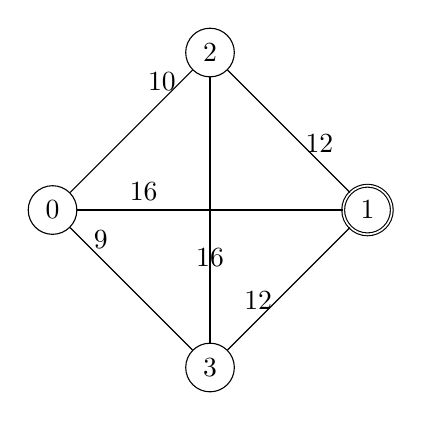
\begin{tikzpicture}[scale=2]
\node[draw,circle] (A) at (0,1) {$2$};
\node[draw,circle,double] (B) at (1,0) {$1$};
\node[draw,circle] (C) at (0,-1) {$3$};
\node[draw,circle] (D) at (-1,0) {$0$};
\foreach \i/\j/\t in {A/B/12,B/C/12,C/D/9,D/A/10,A/C/16,B/D/16} {
  \draw (\i) to node[above,near end]{$\t$} (\j);
}
\end{tikzpicture}